\documentclass[5p,times,twocolumn,authoryear]{elsarticle}
% Two-column Elsevier layout (elsarticle 5p; the Medical Image Analysis format). Bibliography: plainnat (author-year).
% Manuscript v6. Each part lives in sections/*.tex. Build: ./build.sh

\usepackage[OT1]{fontenc} % elsarticle loads T1; OT1 keeps every font Type 1 without cm-super
\usepackage{amsmath,amssymb,amsfonts,bm}
\usepackage{booktabs}
\usepackage{graphicx}
\usepackage{enumitem}
\usepackage{adjustbox}
\usepackage{array}
\usepackage{microtype}
\usepackage{xcolor}
\definecolor{linkblue}{HTML}{335A8A}
\usepackage[colorlinks=true,linkcolor=linkblue,citecolor=linkblue,urlcolor=linkblue]{hyperref}
\usepackage{url}
\usepackage[font=small,labelfont=bf,labelsep=period,skip=4pt]{caption}
\newcolumntype{L}[1]{>{\raggedright\arraybackslash}p{#1}}
\setlist{nosep,leftmargin=*}
\setlength{\emergencystretch}{2.5em}
\renewcommand{\topfraction}{0.9}\renewcommand{\dbltopfraction}{0.9}\renewcommand{\bottomfraction}{0.6}
\renewcommand{\textfraction}{0.07}\renewcommand{\floatpagefraction}{0.75}\renewcommand{\dblfloatpagefraction}{0.75}
\setcounter{topnumber}{4}\setcounter{dbltopnumber}{3}\setcounter{totalnumber}{6}
\makeatletter\g@addto@macro{\UrlBreaks}{\do\-}\makeatother
\biboptions{authoryear,round}
\journal{Medical Image Analysis}

% --- names, fixed once (never typed by hand in the sections) ---
\newcommand{\ms}{\texttt{MedScope-4B}}          % counterfactual training only; the primary model
\newcommand{\msp}{\texttt{MedScope-4B-P}}       % plus pneumothorax films in every stage (post hoc remedy)
\newcommand{\msn}{\texttt{MedScope-4B-N}}       % plus unedited (natural) training images
\newcommand{\base}{\texttt{Qwen3.5-4B}}         % the base model, not fine-tuned
\newcommand{\gem}{\texttt{gemini-4-argon}}
\newcommand{\opus}{\texttt{claude-opus-5-5}}
\newcommand{\gpt}{\texttt{gpt-6-astra}}
\newcommand{\toconfirm}[1]{\textcolor{red}{\textbf{[To confirm: #1]}}}
\newcommand{\ci}[2]{[#1,\,#2]}                  % 95% interval

\begin{document}

% ===================== Front matter (Writer A) =====================
% Every number in the abstract is copied from 04_results_a.tex or 05_results_b.tex; sources are named after it.
\begin{frontmatter}

\title{Vision-language models report lesions erased from medical images: a matched counterfactual evaluation with unedited same-patient pairs}

\author[ind]{Bhaskar Gurram\corref{cor}}
\ead{gurrambhaskar.ai@gmail.com}
\author[ind]{Yoshitha Challagulla}
\author[jc]{Jyothirmaye Challagulla}
\author[shn,uoft]{Samir C. Grover}
\cortext[cor]{Corresponding author.}
\address[ind]{Independent Researcher}
\address[jc]{\toconfirm{affiliation of Jyothirmaye Challagulla (internal medicine)}}
\address[shn]{Scarborough Health Network Research Institute, Toronto, Ontario, Canada}
\address[uoft]{Department of Medicine, University of Toronto, Toronto, Ontario, Canada}

\begin{abstract}
Vision-language models for medical imaging are assessed on unaltered images. However, a correct answer cannot then show that the image was used. We erased lesions from medical images, made matched control edits elsewhere, and asked the same closed question (MedScope-Bench; 507 test cases, five imaging types). The evidence sensitivity gap (ESG), the share of lesions denied after erasure minus that after the control edit, is zero for any constant answer. Nine frontier models reported the finding on 41.1\% to 61.6\% of 219 erased images (ESG 0.269 to 0.470) and on none of 183 blank images, so the question alone did not produce them. \ms, a 4-billion-parameter model trained on such views, reported 9.6\% (95\% confidence interval 6.1 to 13.7; ESG 0.758, 0.701 to 0.815). On 103 unedited same-patient colonoscopy pairs, its analogous gap (natural ESG) equalled its base model's (0.243). \msn, trained also on unedited images, reached 0.612 (0.526 to 0.698) on 116 pairs from a hospital absent from training. It exceeded two comparison models, by 0.310 (0.181 to 0.431) and 0.147 (0.043 to 0.250); a difference from the third, 0.086 ($-0.017$ to 0.190), was not shown. It reported more erased lesions than its predecessor on new external datasets (22.0\% against 11.3\%; difference 0.107, 0.054 to 0.162). On public images with closed questions, the models tested often reported lesions no longer shown. Counterfactual training reduced such reports in one small model; detection on unedited images required unedited training images. Complete specialist reading of the erasures and prospective evaluation are needed.
\end{abstract}
% src: 04_results_a.tex subsec:res_main (507 cases; 41.1-61.6% of 219; ESG 0.269-0.470; 9.6% [6.1, 13.7]; 0.758 [0.701, 0.815]; blank image 0% of 183 = L1784-1805);
%      05_results_b.tex subsec:res_pairs (103 pairs, 0.243 for both; 116 pairs, 0.612 [0.526, 0.698]; +0.147 [+0.043, +0.250]; +0.310 [+0.181, +0.431]; +0.086 [-0.017, +0.190] = L2145-2159);
%      05_results_b.tex subsec:res_nmodel (22.0% against 11.3%, +0.107 [+0.054, +0.162] = L2178-2183); 03_methods.tex subsec:models (about 4 billion parameters)

\begin{keyword}
vision-language models \sep medical imaging \sep counterfactual evaluation \sep inpainting \sep evidence sensitivity \sep reader study \sep colonoscopy
\end{keyword}

\end{frontmatter}

% 01_introduction: to be written

% ===================== 2. Related work (Writer A) =====================
% No results of this study. Numbers of prior studies carry a "% src:" line; numbers that the Discussion compares with ours
% are given there only. Descriptions of prior work follow writing_study/group3_vlm_benchmarks.md ("How the closest prior
% work describes itself"), group2 (RadEdit) and v5 P407-447.
\section{Related work}\label{sec:related}

\textit{Changing the question.} Most tests of whether a VLM reports a finding that is absent change the question and leave the image as it is. POPE asks balanced yes/no questions about objects that are or are not in a photograph \citep{li2023pope}. ProbMed pairs each true question about a medical image with an adversarial question that names an invented finding or attribute, and scores the pair only when both answers are right \citep{yan2024probmed}. CARES, Med-HallMark and MedHEval grade answers or generated text about unaltered medical images over wider sets of properties \citep{xia2024cares,chen2024medhallmark,chang2024medheval}. \citet{jin2024hidden} had physicians read the rationales of one model and found flawed rationales behind many correct answers, most often in image comprehension. In all of these studies the image is held fixed, so a correct ``no'' cannot be attributed to the image.
% src: writing_study/papers_g3/jin_npj.md L22, L101 (category "image comprehension"; the numbers are given in the Discussion); group3 notes (POPE, ProbMed, CARES, Med-HallMark); v5 P405 (MedHEval)

\textit{Changing the image.} A second group holds the question fixed and changes the whole image. MedVH replaces a chest radiograph with an unrelated image \citep{gu2024medvh}, and \citet{gu2025illusion} remove the image from multiple-choice cases or substitute one that fits another answer option. The closest work is that of \citet{lotfinia2026image}. They exchanged a chest radiograph for another patient's with the same or the opposite label, occluded the radiologist-marked region or an equal region elsewhere, and had radiologists read the same altered images. A language model given only the question scored $55.3\%$ on their pooled questions, above two multimodal systems. The authors state that their swaps are not minimal pairs, and that images which remove the finding and preserve the image statistics would be more faithful. Such paired edits exist for general images \citep{agarwal2020towards}: HallusionBench pairs an original with a hand-edited image for which the correct answer differs \citep{guan2024hallusionbench}. In medical imaging, RadEdit edits chest radiographs with a diffusion model to stress-test classifiers and segmentation models \citep{perez2024radedit}, and HEAL-MedVQA swaps the queried anatomical region of a chest radiograph \citep{healmedvqa2024}. Recent preprints replace the whole image \citep{zafar2026coral}, exchange tumour intensities between MRI sequences \citep{sun2026prive}, or build counterfactuals from image features or local perturbations \citep{huang2026medcap,lin2026medcausalx}. None of the studies that edit the image content (RadEdit and those listed after it in Table~\ref{tab:related}) pairs a lesion-shaped erasure with an edit of the same shape and tool elsewhere in the same image, or reports an assessment of the edited images by clinicians.
% src: writing_study/papers_g3/lotfinia_main.md (L23, L25: 55.3% text-only, higher than two multimodal systems; L311, L328-330: not minimal pairs, finding-removing counterfactuals more faithful); group3 notes (MedVH, The Illusion of Readiness, HallusionBench); group2 notes (RadEdit); v5 P409-413 (Agarwal et al., HEAL-MedVQA, CORAL, PriVE-Bench, Med-CAP, MedCausalX)

\textit{Training remedies.} Similar pairs have been used for training. MMedPO adds noise to lesion regions to build the rejected side of preference pairs \citep{zhu2024mmedpo}. Several methods train general VLMs on minimal-pair or contrasting images with preference optimisation \citep{svco2024,wu2025empo,jiang2025mfpo,rafailov2023dpo}, and CORAL penalises answers that stay the same when the image is replaced \citep{zafar2026coral}. These methods are evaluated by accuracy, or by the rate of unsupported statements, on benchmarks of unaltered images. Such measures do not separate answering ``absent'' more often from answering ``absent'' when the finding is absent. A matched control edit does, because a model that answers ``absent'' more often also does so when the lesion is intact. The present study applies this control to a trained model and to the models it is compared with, and adds a test on unedited image pairs.
% src: v5 P415-421, P437-439 (MMedPO, S-VCO, EMPO, MFPO, CORAL and how each is validated); no numbers

\begin{table*}[!t]
\caption{Design features of the closest prior work and of this study, taken from the published descriptions. Yes: the feature is present. Partly: present in the restricted form given in the note. No: absent. --: not applicable. Not stated: not stated in the sources consulted. Works are ordered as in the text.}
\label{tab:related}
\centering
\footnotesize
\setlength{\tabcolsep}{3pt}
\renewcommand{\arraystretch}{1.05}
\begin{tabular}{@{}L{0.27\textwidth}*{7}{>{\centering\arraybackslash}p{0.088\textwidth}}@{}}
\toprule
\textbf{Study} & \textbf{Medical images} & \textbf{Image varied, question fixed} & \textbf{Edit confined to the finding} & \textbf{Matched control edit} & \textbf{Altered images assessed by clinicians} & \textbf{Unedited same-patient pairs} & \textbf{Trained remedy} \\
\midrule
ProbMed \citep{yan2024probmed} & Yes & No & -- & -- & -- & No & No \\
MedVH \citep{gu2024medvh} & Yes & Yes$^{a}$ & No & No & No & No & No \\
\citet{gu2025illusion} & Yes & Yes$^{a}$ & No & No & Yes$^{b}$ & No & No \\
\citet{lotfinia2026image} & Yes & Yes & Partly$^{c}$ & Yes$^{d}$ & Yes & No$^{e}$ & No \\
HallusionBench \citep{guan2024hallusionbench} & No & Yes & Partly$^{f}$ & No & -- & No & No \\
RadEdit \citep{perez2024radedit} & Yes & Yes$^{g}$ & Yes & No & No & No & No \\
HEAL-MedVQA \citep{healmedvqa2024} & Yes & Yes & Partly$^{h}$ & No & No & Not stated & Yes \\
PriVE-Bench \citep{sun2026prive} & Partly$^{i}$ & Yes & Partly$^{i}$ & No & No & Not stated & Not stated \\
MMedPO \citep{zhu2024mmedpo} & Yes & No$^{j}$ & Partly$^{j}$ & No & No & Not stated & Yes \\
CORAL \citep{zafar2026coral} & Yes & Yes$^{a}$ & No & No & No & Not stated & Yes \\
\midrule
This study & Yes & Yes & Yes & Yes & Partly$^{k}$ & Yes$^{l}$ & Yes \\
\bottomrule
\multicolumn{8}{@{}p{0.97\textwidth}@{}}{$^{a}$\,The whole image is removed or replaced. $^{b}$\,Clinicians verified that each substituted image supported the new answer. $^{c}$\,The radiologist-marked region is occluded, not removed. $^{d}$\,An equal region occluded elsewhere, and a swap with a radiograph of the same label. $^{e}$\,Swaps use unedited radiographs of other patients. $^{f}$\,Hand edits of general images (charts, maps, illusions). $^{g}$\,Classification and segmentation models; no questions are asked. $^{h}$\,The queried anatomical region is swapped in from another radiograph. $^{i}$\,One of five domains is medical: tumour-region intensities exchanged between MRI sequences. $^{j}$\,Noise in lesion regions, used to build training pairs; evaluation uses unaltered images. $^{k}$\,Two trainee physicians (all imaging types), a board-certified radiologist and a board-certified gastroenterologist (Section~\ref{subsec:res_readers}). $^{l}$\,Colonoscopy frames, and chest X-ray follow-up pairs as a secondary analysis; the pneumothorax films are unedited but not paired by patient.} \\
\end{tabular}
\end{table*}
% src: group3 notes, section "How the closest prior work describes itself" (ProbMed, MedVH, The Illusion of Readiness, Lotfinia et al., HallusionBench); group2 notes section 8 (RadEdit); v5 P423-447 (table of closest work: control and reader columns for HEAL-MedVQA, RadEdit, MMedPO, CORAL, PriVE-Bench). Cells that neither source supports are "Not stated". The column on editing tools not used in training was dropped (only this study could fill it).

% 03_methods: to be written

% 04_results_a: to be written

% 05_results_b.tex  (Writer D)  Results, part 2: Sections 4.6-4.8. Continues \section{Results} of 04_results_a.tex.
% Every number is copied from docs/RESULTS_LOG.md (L = line), the fact sheet (facts), the stored report of the
% final run (report60 = scratchpad/report60.md, line numbers) or paper/v5/paper.tex (v5 P = line).
% Template (round 2): shares in per cent; differences between shares in percentage points (stored proportion
% difference and its bounds times 100, nothing else); ESG, natural ESG and Youden index on the 0 to 1 scale;
% positive differences unsigned.

\subsection{Unedited image pairs: the advantage did not carry over, and detection improved only with unedited training images}
\label{subsec:res_pairs}

On 103 unedited pairs from REAL-Colon, a polyp frame and a polyp-free frame of the same video received the same question (Section~\ref{subsec:pairs}). The natural ESG of \ms{} was $0.243$ $\ci{0.149}{0.340}$, the same as that of its base model (difference $0.000$ $\ci{-0.103}{0.095}$) and lower than that of \gem{} ($0.466$; $-0.223$ $\ci{-0.346}{-0.102}$) and \opus{} ($0.447$; $-0.204$ $\ci{-0.333}{-0.071}$); the pre-specified criterion was not met (Table~\ref{tab:natural}; Supplementary Table~\ref{tab:s_realcolon}). \ms{} reported a polyp on 2 of 103 polyp-free frames, against 15 for its base model, but it requested a better image on 12 more, and the share answered ``absent'' or referred was the same (86.4\% against 85.4\%). It reported the polyp on 36 of 103 polyp frames, against 40.
% src: L1458-1468 (natural ESG, differences, criterion); L1484-1489 (2/103, 15/103, 12 requests, 89/103 = 86.4%, 36/103, 40/103)

A two-by-two comparison of first-stage models, trained with or without counterfactual views and with or without unedited pairs, separated the two kinds of training image (one seed; Supplementary Table~\ref{tab:s_twobytwo}). Natural ESG was $0.563$ with unedited pairs only, $0.505$ with both kinds, $0.223$ with counterfactual views only and $0.214$ with neither. Unedited pairs raised it by $0.350$ $\ci{0.227}{0.474}$ without counterfactual views and by $0.282$ $\ci{0.156}{0.405}$ with them. Counterfactual views were not shown to add to it once unedited pairs were in training ($-0.058$ $\ci{-0.168}{0.042}$, $p = 0.311$; the pre-specified comparison). Without unedited pairs, they raised the share of polyp-free frames answered ``absent'' or referred (86.4\% against 68.9\%; a polyp reported on 3 against 27 of 103) and lowered the share of polyp frames found (35.9\% against 52.4\%). On the main test, ESG was $0.744$ with both kinds and $0.260$ with unedited pairs only (difference $0.484$ $\ci{0.408}{0.558}$).
% src: L1997-2026; facts C7 (two-by-two table: found 35.9% and 52.4%, absent or referred 86.4% and 68.9%, polyp reported 3 and 27) and C1 (main test)

\begin{table*}[!t]
\caption{Unedited colonoscopy pairs: a polyp frame and a polyp-free frame of the same video or clip, both asked ``Is there a polyp in this image?''. REAL-Colon: 103 pairs from 46 videos of four centres; the answers of \msn{} are cross-validated (each pair is answered by a copy trained without that pair's video). LDPolypVideo: 116 pairs from 160 clips of one hospital, none of whose images was used to train or select any of our models. Found: the polyp frame was not answered ``absent'' and was not referred; a request for a better image therefore counts as found. Absent or referred: the answer to the polyp-free frame. Natural ESG: the share of polyp-free frames answered ``absent'' or referred minus the same share for polyp frames. Brackets give 95\% intervals from $2{,}000$ bootstrap resamples of whole videos or clips. Differences are \msn{} minus the row model, paired over the same pairs, with two-sided $p$ values. \msn{} is the model of the first training seed; the majority vote of its three seeds scored $0.586$ $\ci{0.491}{0.673}$ on LDPolypVideo. The differences of \ms{} from the other models on REAL-Colon are in Supplementary Table~\ref{tab:s_realcolon}. --: not applicable.}
\label{tab:natural}
\centering
\footnotesize
\setlength{\tabcolsep}{3.5pt}
\begin{adjustbox}{max width=\textwidth}
\begin{tabular}{l cccc cccc}
\toprule
 & \multicolumn{4}{c}{REAL-Colon ($103$ pairs)} & \multicolumn{4}{c}{LDPolypVideo ($116$ pairs)} \\
\cmidrule(lr){2-5}\cmidrule(lr){6-9}
Model & \shortstack{Polyp\\frames\\found} & \shortstack{Polyp-free\\frames absent\\or referred} & \shortstack{Natural ESG\\{}[95\% CI]} & \shortstack{\msn{} minus model\\{}[95\% CI], $p$} & \shortstack{Polyp\\frames\\found} & \shortstack{Polyp-free\\frames absent\\or referred} & \shortstack{Natural ESG\\{}[95\% CI]} & \shortstack{\msn{} minus model\\{}[95\% CI], $p$} \\
\midrule
\base{} & $38.8\%$ & $85.4\%$ & $0.243$ $\ci{0.143}{0.350}$ & $0.291$ $\ci{0.167}{0.407}$, $<0.001$ & $40.5\%$ & $95.7\%$ & $0.362$ $\ci{0.276}{0.448}$ & $0.250$ $\ci{0.155}{0.353}$, $<0.001$ \\
\ms{} & $37.9\%$ & $86.4\%$ & $0.243$ $\ci{0.149}{0.340}$ & $0.291$ $\ci{0.176}{0.402}$, $<0.001$ & $45.7\%$ & $96.6\%$ & $0.422$ $\ci{0.328}{0.517}$ & $0.190$ $\ci{0.112}{0.267}$, $<0.001$ \\
\msn{} & $64.1\%$ & $89.3\%$ & $0.534$ $\ci{0.394}{0.661}$ & -- & $62.1\%$ & $99.1\%$ & $0.612$ $\ci{0.526}{0.698}$ & -- \\
\midrule
\gem{} & $68.0\%$ & $78.6\%$ & $0.466$ $\ci{0.336}{0.581}$ & $0.068$ $\ci{-0.069}{0.202}$, $0.347$ & $71.6\%$ & $81.0\%$ & $0.526$ $\ci{0.422}{0.621}$ & $0.086$ $\ci{-0.017}{0.190}$, $0.117$ \\
\opus{} & $70.9\%$ & $73.8\%$ & $0.447$ $\ci{0.317}{0.579}$ & $0.087$ $\ci{-0.049}{0.230}$, $0.259$ & $62.9\%$ & $83.6\%$ & $0.466$ $\ci{0.362}{0.569}$ & $0.147$ $\ci{0.043}{0.250}$, $0.010$ \\
\gpt{} & $64.1\%$ & $68.0\%$ & $0.320$ $\ci{0.212}{0.437}$ & $0.214$ $\ci{0.071}{0.343}$, $0.003$ & $55.2\%$ & $75.0\%$ & $0.302$ $\ci{0.198}{0.405}$ & $0.310$ $\ci{0.181}{0.431}$, $<0.001$ \\
\bottomrule
\end{tabular}
\end{adjustbox}
\end{table*}
% src: REAL-Colon columns report60 L117-126 (= L1458-1465, L2162-2165); LDPolypVideo columns report60 L69-80 (= L2145-2156); vote report60 L74; a p value of 0.000 in the report is printed as < 0.001

\msn{} is a post hoc model: \msp{} with unedited colonoscopy frames and chest films added to its training (Section~\ref{subsec:models}). On 116 pairs from LDPolypVideo, a hospital not used to train or select our models, it answered ``absent'' or referred on 99.1\% of the polyp-free frames, against 75.0\% to 83.6\% for the reference models, while finding 62.1\% of the polyp frames (reference models 55.2\% to 71.6\%; Fig.~\ref{fig:natural}). Its natural ESG was $0.612$ $\ci{0.526}{0.698}$, higher than that of \ms{} ($0.422$; difference $0.190$ $\ci{0.112}{0.267}$, $p < 0.001$), \opus{} ($0.466$; $0.147$ $\ci{0.043}{0.250}$, $p = 0.010$) and \gpt{} ($0.302$; $0.310$ $\ci{0.181}{0.431}$, $p < 0.001$). A difference from \gem{} ($0.526$) was not shown ($0.086$ $\ci{-0.017}{0.190}$, $p = 0.117$), so by the pre-specified rule the result is mixed. The other two training seeds scored $0.578$ and $0.578$ (Supplementary Table~\ref{tab:s_ldpolyp}).
% src: L2145-2159; facts C9; report60 L69-80 (seeds 1 and 2: 0.578, 0.578); verdict "MIXED" L2145

\begin{figure*}[!t]
\centering
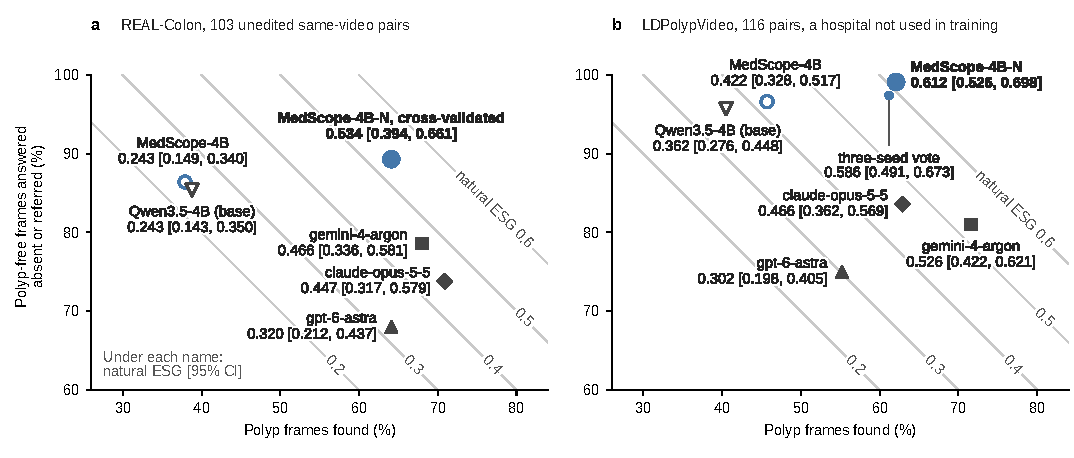
\includegraphics[width=\textwidth]{figures/fig4_natural_pairs.pdf}
\caption{Unedited colonoscopy pairs, by model. (a) REAL-Colon, 103 pairs from 46 videos; the answers of \msn{} are cross-validated. (b) LDPolypVideo, 116 pairs from 160 clips of a hospital not used to train or select any of our models. Each point places a model by the share of polyp frames it found (not answered ``absent'' and not referred, so a request for a better image counts as found) and the share of polyp-free frames it answered ``absent'' or referred. Natural ESG is the sum of the two shares minus one; grey diagonals join points of equal natural ESG, and the value under each name is the natural ESG with its 95\% interval ($2{,}000$ bootstrap resamples of whole videos or clips). The small filled circle in (b) is the three-seed majority vote of \msn{}. Values are in Table~\ref{tab:natural}.}
\label{fig:natural}
\end{figure*}
% src: same numbers as Table tab:natural

On the REAL-Colon pairs, which had already been used to test \ms{}, cross-validated \msn{} scored $0.534$ $\ci{0.394}{0.661}$. This was higher than \ms{} (difference $0.291$ $\ci{0.176}{0.402}$, $p < 0.001$) and \gpt{} ($0.214$ $\ci{0.071}{0.343}$, $p = 0.003$) and not shown to differ from \gem{} ($0.068$ $\ci{-0.069}{0.202}$, $p = 0.347$) or \opus{} ($0.087$ $\ci{-0.049}{0.230}$, $p = 0.259$). An earlier model with only the colonoscopy frames added scored $0.495$ $\ci{0.370}{0.612}$ when every video of the tested centre was withheld from training; context-matched frames and chest X-ray follow-up pairs are in Supplementary Tables~\ref{tab:s_loco} to~\ref{tab:s_cxrpairs}.
% src: L2162-2165; report60 L119-126; L1867-1869 (centre withheld: 0.495 [0.370, 0.612])

\subsection{\texorpdfstring{\msn}{MedScope-4B-N} on the earlier tests and on chest films}
\label{subsec:res_nmodel}

On the main test \msn{} was not shown to differ from \ms{}: ESG was $0.744$ against $0.758$ (difference $-0.014$ $\ci{-0.068}{0.040}$). The pre-specified criterion for a loss, an ESG lower by more than $0.05$, was not met, although the interval does not exclude a fall of that size (Table~\ref{tab:nmodel}). Each of its three training seeds exceeded each reference model in ESG ($0.744$, $0.740$ and $0.726$; smallest difference $0.256$ $\ci{0.171}{0.338}$; Supplementary Table~\ref{tab:s_nseeds}). On the external datasets its ESG was higher than that of \ms{} ($0.672$ against $0.597$; difference $0.076$ $\ci{0.009}{0.143}$, $p = 0.033$) and lower than that of \msp{} ($0.739$; $-0.067$ $\ci{-0.126}{-0.009}$, $p = 0.025$).
% src: L2141-2143; report60 L24, L226 (main test); L2127-2139, report60 L461 (seeds; smallest difference: third seed minus gemini-4-argon); L2185-2186, report60 L291, L296 (external datasets)

On the fresh external set \msn{} was correct on more lesion images than \ms{} (60.7\% against 47.6\%; difference 13.1 percentage points $\ci{6.9}{19.7}$) and reported 22.0\% of erased lesions, against 11.3\% for \msp{} (difference 10.7 percentage points $\ci{5.4}{16.2}$) and 8.3\% for \ms{} (13.7 $\ci{7.7}{20.2}$). The increase was largest on chest films (33\% against 10\%; by source in Supplementary Table~\ref{tab:s_source}), and the training mix that validation did not select reported 17.3\%. Beside \gem{} on this set, \msn{} reported fewer erased lesions (22.0\% against 31.5\%), had a lower ESG ($0.381$ against $0.435$) and was correct on fewer lesion images (60.7\% against 74.1\%); these three contrasts were not tested.
% src: L2178-2183, L2189-2191; report60 L267-268, L273 (0.131 [0.069, 0.197]; 0.137 [0.077, 0.202]; 0.107 [0.054, 0.162], each times 100), L340-347 (chest films 0.33 against 0.10); gemini-4-argon on the fresh external set: L1683 and v5 P1367 (lesion images correct 0.741, ESG 0.435, erased-lesion claims 31.5%)

On unedited chest films \msn{} exceeded all three reference models. On 300 pneumothorax films and 300 films without pneumothorax from CheXthought, from patients not used in training and from the source of part of its training films, its Youden index was $0.660$ $\ci{0.591}{0.726}$. The reference models scored $0.460$, $0.207$ and $0.377$ (differences $0.200$ $\ci{0.122}{0.284}$, $0.453$ $\ci{0.344}{0.560}$ and $0.283$ $\ci{0.196}{0.375}$ for \gem{}, \opus{} and \gpt{}; each $p < 0.001$). Pneumothorax detection on new SIIM-ACR patients, a test used before with the earlier models, was not raised over \msp{} by the first seed (54 against 53 of 100; difference 1.0 percentage point $\ci{-8.0}{10.0}$). The other seeds found 75 and 70, with more reports on erased films (25.0\%, 59.0\% and 43.0\% for the three seeds).
% src: L2174-2176, facts C6, report60 L206-216 (CheXthought); L2169-2172, report60 L22, L196 (0.010 [-0.080, 0.100] times 100), L405-411 (erased-lesion claims by seed on new SIIM-ACR patients: 0.250, 0.590, 0.430)

\begin{table*}[!t]
\caption{\ms{}, the post hoc model \msn{} and \gem{} on each test set. Point estimates; intervals, paired differences, \msp{} and the three-seed vote are in Supplementary Tables~\ref{tab:s_nmodel}, \ref{tab:s_nseeds} and~\ref{tab:s_chest}. ESG: evidence sensitivity gap. Lesion images correct: share of original and control-edited lesion images answered correctly; for the two sets of chest films this column gives the share of unedited pneumothorax films reported as showing a pneumothorax. Youden index: that share plus the share of films without pneumothorax answered ``absent'' or referred, minus one. The CheXthought films have no erased version. --: not applicable, or model not run on the set.}
\label{tab:nmodel}
\centering
\footnotesize
\setlength{\tabcolsep}{4pt}
\begin{adjustbox}{max width=\textwidth}
\begin{tabular}{l ccc ccc ccc ccc}
\toprule
 & \multicolumn{3}{c}{ESG} & \multicolumn{3}{c}{Erased-lesion claims} & \multicolumn{3}{c}{Lesion images correct} & \multicolumn{3}{c}{Youden index} \\
\cmidrule(lr){2-4}\cmidrule(lr){5-7}\cmidrule(lr){8-10}\cmidrule(lr){11-13}
Test set & \ms{} & \msn{} & \gem{} & \ms{} & \msn{} & \gem{} & \ms{} & \msn{} & \gem{} & \ms{} & \msn{} & \gem{} \\
\midrule
Main test ($507$ cases) & $0.758$ & $0.744$ & $0.470$ & $9.6\%$ & $9.1\%$ & $41.1\%$ & $84.9\%$ & $84.7\%$ & $87.4\%$ & -- & -- & -- \\
External datasets ($169$ cases) & $0.597$ & $0.672$ & $0.370$ & $11.8\%$ & $10.9\%$ & $58.8\%$ & $72.7\%$ & $77.7\%$ & $95.0\%$ & -- & -- & -- \\
Fresh internal set ($76$ cases) & $0.472$ & $0.417$ & $0.056$ & $19.4\%$ & $25.0\%$ & $61.1\%$ & $68.1\%$ & $68.1\%$ & $63.9\%$ & -- & -- & -- \\
Fresh external set ($316$ cases) & $0.393$ & $0.381$ & $0.435$ & $8.3\%$ & $22.0\%$ & $31.5\%$ & $47.6\%$ & $60.7\%$ & $74.1\%$ & -- & -- & -- \\
New SIIM-ACR patients ($100 + 100$ films) & $0.000$ & $0.270$ & -- & $0.0\%$ & $25.0\%$ & -- & $0$ of $100$ & $54$ of $100$ & -- & $0.000$ & $0.500$ & -- \\
CheXthought test patients ($300 + 300$ films) & -- & -- & -- & -- & -- & -- & $0.0\%$ & $75.0\%$ & $62.0\%$ & $0.000$ & $0.660$ & $0.460$ \\
\bottomrule
\end{tabular}
\end{adjustbox}
\end{table*}
% src: MedScope-4B and MedScope-4B-N: Supplementary Table tab:s_nmodel (report60 L225-228, L265-268, L290-293, L310-313; lesion images correct and claims are the report's proportions times 100); new SIIM-ACR patients: report60 L190, L197, L407-411 and L1600-1602 (MedScope-4B: ESG 0.000, erased-lesion claims 0.000); CheXthought: report60 L206, L212, L214. gemini-4-argon: main test L486-493 (facts C: 0.874, 0.470, 41.1%); external datasets, fresh internal and fresh external v5 P1359, P1363, P1367 (0.950, 0.370, 58.8; 0.639, 0.056, 61.1; 0.741, 0.435, 31.5; = L1683 for the fresh external set)

\subsection{Alternative training designs and decision rules}
\label{subsec:res_designs}

Seventeen alternative designs were each tested against a criterion fixed in advance, and none met it (Supplementary Tables~\ref{tab:s_designs}, \ref{tab:s_designs_later} and~\ref{tab:s_inspect}; Supplementary Fig.~\ref{fig:s_designs}). They changed the training objective, the adapter, the system design, the mix of editing tools in training or the answer score at decision time. Matching the control edit to the erasure in shape and tool during training was not shown to matter (inconclusive under its rule), and counterfactual training was not shown to exceed preference optimisation on the fresh external set (ESG $0.381$ against $0.355$, means of three seeds). One design lowered ESG to $0.000$; the other recorded changes in ESG lay between $-0.054$ and $0.041$, and several designs had one seed, so small gains are not excluded. None of 270 decision rules passed on both halves of the validation set.
% src: count: twelve rows of tab:s_designs + three of tab:s_designs_later + two of tab:s_inspect = seventeen; v5 P752 (range -0.054 to +0.041), P767-772, P927 (one seed), P1263-1288; L883-886 (matching inconclusive); L916-922 (0.381 +- 0.018 vs 0.355 +- 0.015, three seeds); L1058-1060 (ESG 0.000 on every set for the vision-encoder adapter at the higher learning rate); L1184-1205 (270 rules: 19 of 128 passed on one half, none on both; 0 of 142)

% 06_discussion: to be written

% 07_backmatter: to be written


\bibliography{refs}
\bibliographystyle{plainnat}

\newpage
\onecolumn
\appendix
\setcounter{table}{0}\renewcommand{\thetable}{S\arabic{table}}
\setcounter{figure}{0}\renewcommand{\thefigure}{S\arabic{figure}}
% supp_a_plan_methods: to be written

% supp_b_results_a: to be written

% supp_c_results_b: to be written

% ===================== Supplement D: reporting checklist (Writer A) =====================
% The table of paper/v5/paper.tex lines 1135-1174 with every pointer updated to the sections and labels of this version.
\section{Reporting checklist}\label{sec:s_claim}

Table~\ref{tab:s_claim} maps the manuscript to the Checklist for Artificial Intelligence in Medical Imaging (CLAIM) \citep{mongan2020claim}, 2024 update \citep{tejani2024claim}, grouped by the sections of the checklist.
% src: v5 P1137

\begin{table}[!htbp]
\caption{Where each part of the CLAIM 2024 checklist is addressed. ESG: evidence sensitivity gap. LoRA: low-rank adapter.}
\label{tab:s_claim}
\centering
\small
\renewcommand{\arraystretch}{1.12}
\begin{tabular}{@{}L{0.25\textwidth}L{0.71\textwidth}@{}}
\toprule
\textbf{Checklist section} & \textbf{Where and how it is addressed} \\
\midrule
Title, abstract & Title; abstract (design, data, main results with intervals, and the comparison that was not shown). \\
Introduction: background, objectives, hypotheses & Section~\ref{sec:intro}: the clinical setting, the logical limit of accuracy on unaltered images, four requirements for an intervention on the finding, and the aim. Predictions for a model that uses the image and for one that does not: Section~\ref{subsec:design}. \\
Study design and intended use & Retrospective study of public, de-identified datasets. A benchmark and research models, not a clinical device (Sections~\ref{subsec:design} and~\ref{subsec:data}; Table~\ref{tab:overview}). \\
Data sources, selection, preprocessing & Sources and counts (Section~\ref{subsec:data}, Table~\ref{tab:datasets}); lesions smaller than 20 pixels or larger than 20\% of the image excluded; closed questions; automated checks of the edited views (Section~\ref{subsec:views}, \ref{sec:s_views}); long side of every image at most 768 pixels (Section~\ref{subsec:models}). \\
De-identification & Public releases, de-identified by their providers; no new patient data were collected; the reader study used the same images. \\
Missing data & Cases that failed an automated check or an edit were dropped with both edited views; exclusions before splitting are counted in \ref{sec:s_plan}. Analyses on fewer cases state the number kept and the reason: 125 cases with valid views for all four editing tools, 116 of 160 clips with an unedited pair, 183 of 200 chest X-ray follow-up pairs (Sections~\ref{subsec:data} and~\ref{subsec:pairs}, \ref{sec:s_views}). \\
Imaging parameters & As released by each source; not available per image and not analysed (Section~\ref{sec:discussion}, limitation iv). \\
Reference standard & Expert lesion masks and labels of the source datasets. For an erased image, absence by construction, assessed by a specialist reader round that is still open and by an earlier trainee round (Sections~\ref{subsec:measures}, \ref{subsec:readers} and~\ref{subsec:res_readers}; \ref{sec:s_readers}). \\
Data partitions and independence & Splits by patient or by group of near-identical images, made before any view was built; hash comparison of all images across sets; an analysis without the test cases most similar to a training image; cross-validated answers where a source serves in training and in testing (Sections~\ref{subsec:data}, \ref{subsec:models} and~\ref{subsec:res_alternatives}). \\
Test-set size & Set by the available cases and fixed in advance, not by a power calculation (Sections~\ref{subsec:data} and~\ref{subsec:pairs}). \\
Model, software, initialization & \base{} with a LoRA adapter of rank 16 and a frozen vision encoder, initialized from the public base model; software versions (Sections~\ref{subsec:models} and~\ref{subsec:stats}; \ref{sec:s_plan}). \\
Training and model selection & Three training stages and a selection rule fixed in advance for \ms; \msp{} and \msn{} post hoc, each with a validation rule fixed before its test results; three training seeds; a three-seed majority vote reported next to the single model (Section~\ref{subsec:models}; Supplementary Tables~\ref{tab:s_models} and~\ref{tab:s_mix}). \\
Metrics and statistics & ESG, erased-lesion claims, lesion-free claims, lesion images correct, net utility, natural ESG and Youden index, each with the value a constant answer earns (Section~\ref{subsec:measures}); bootstrap over cases, videos or patients, paired comparisons, Bonferroni correction over 27 primary comparisons (Section~\ref{subsec:stats}). \\
Robustness and interpretability & Prompting conditions, question wordings, cost matrices, editing tools, lesion size and training seeds (Sections~\ref{subsec:res_main} and~\ref{subsec:res_alternatives}; Supplementary Tables~\ref{tab:s_prompts}, \ref{tab:s_sensitivity}, \ref{tab:s_cost}, \ref{tab:s_tools}, \ref{tab:s_size} and~\ref{tab:s_seeds}); probes of hidden states (Supplementary Table~\ref{tab:s_site}). \\
Internal and external testing & Main test; external centres, fresh internal and fresh external sets (Section~\ref{subsec:res_external}, Supplementary Table~\ref{tab:s_external}); unedited same-patient pairs, including a hospital not used in training (Section~\ref{subsec:res_pairs}); chest films (Section~\ref{subsec:res_nmodel}). \\
Registration & The analysis plan is a set of dated files in the public project repository, the authors' own record and not a third-party registry (Section~\ref{subsec:stats}, Supplementary Table~\ref{tab:s_plan}). The study is not a clinical trial. \\
Data flow and demographics & Counts per source and per evaluation set (Table~\ref{tab:datasets}); demographics were not compiled (Section~\ref{sec:discussion}, limitation iv). \\
Performance and errors & Tables with intervals; results by imaging type, editing tool and lesion size (Supplementary Tables~\ref{tab:s_modality}, \ref{tab:s_tools} and~\ref{tab:s_size}); a counted analysis of the pneumothorax miss (Section~\ref{subsec:res_external}); model answers scored again on erasures that readers called clean (Section~\ref{subsec:res_readers}). \\
Discussion & What the results do and do not show, limitations and the evidence still needed (Section~\ref{sec:discussion}). \\
Protocols, code, data & Data and code availability statement: analysis plan, code, models and stored model answers. \\
Funding & No external funding. \\
\bottomrule
\end{tabular}
\end{table}
% src: v5 P1139-1174 (checklist rows); pointers and facts from 03_methods.tex (subsec:data: 20 pixels, 20%; subsec:models: 768 pixels, rank 16; subsec:stats: 27 comparisons), 04_results_a.tex and 05_results_b.tex (125 cases; 116 of 160 clips; 183 of 200 pairs)


\end{document}
